\documentclass[12pt]{article}
\usepackage{setspace,graphicx,amsmath,geometry,fontspec,titlesec,soul,bm,subfigure}
\titleformat{\section}[block]{\LARGE\bfseries}{\arabic{section}}{1em}{}[]
\titleformat{\subsection}[block]{\Large\bfseries\mdseries}{\arabic{section}.\arabic{subsection}}{1em}{}[]
\titleformat{\subsubsection}[block]{\normalsize\bfseries}{\arabic{subsection}-\alph{subsubsection}}{1em}{}[]
\titleformat{\paragraph}[block]{\small\bfseries}{[\arabic{paragraph}]}{1em}{}[]
\setmainfont{Times New Roman}
\renewcommand{\baselinestretch}{1.15}
\geometry{a4paper,left=2.5cm,right=2.5cm,top=2.5cm,bottom=2.5cm}
\begin{document}
	\newpagestyle{main}{            
		\sethead{Ziqing Yu}{Bildverarbeitung 5}{3218051}     
		\setfoot{}{\thepage}{}
		\headrule
		\footrule
			}
	\pagestyle{main}
\section{Einleitung}
In dieser Übung sind 2 Bilder mit den zugehörigen Parametern der inneren und äußeren Orientierung sowie die Koordinaten signalisierter Punkte zur Verfügung. Eine Vorwärtsschnitt wird durchgeführt. \newline
\section{Vorwärtsschnitt}
Zurerst sind Pixelkoordinaten eines beliebigen Objektpunkts in den Bildern mit MATLAB-Programm imtool zu bestimmen, zur Kontrolle sind die Koordinaten des signalisierten Punktes P25 genutzt: 
\begin{figure*}[ht]\centering
	\subfigure[P25 auf Bild 1]{
		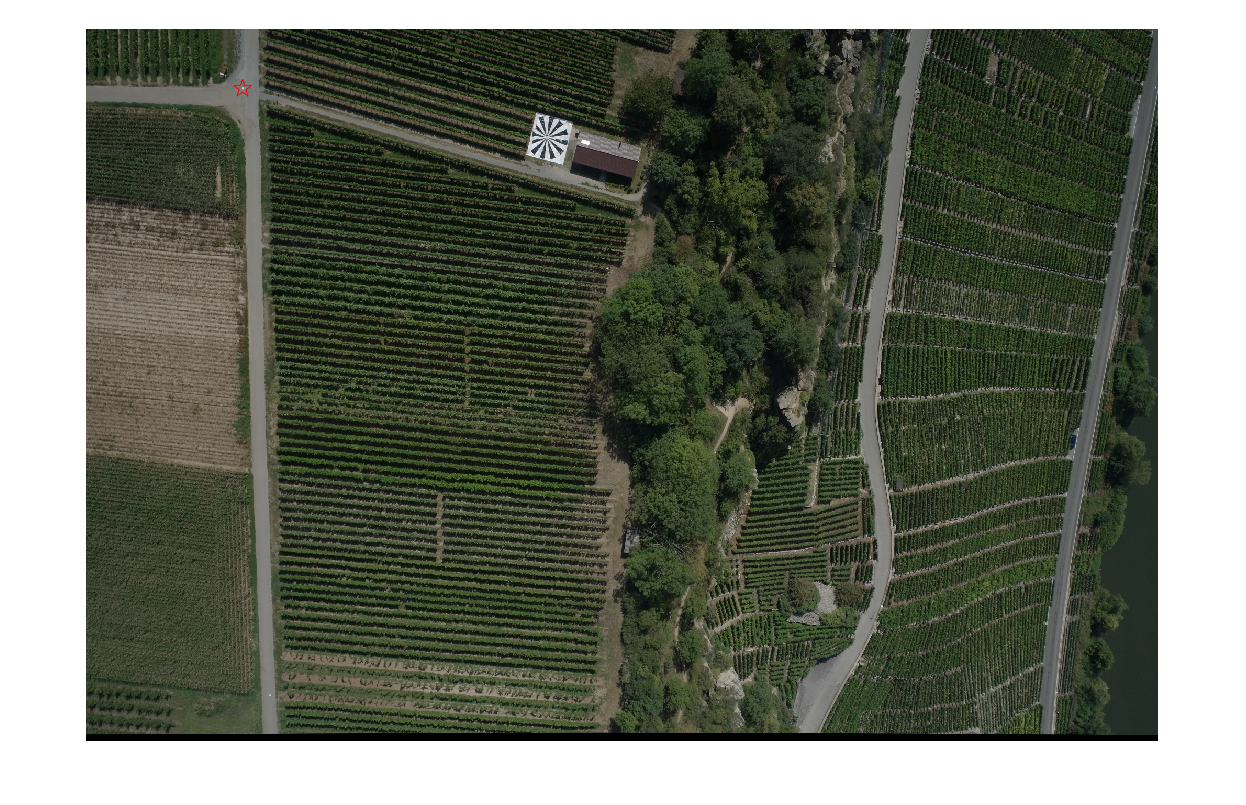
\includegraphics[width=0.45\textwidth]{P1.png}}
	\subfigure[P25 auf Bild 2]{
		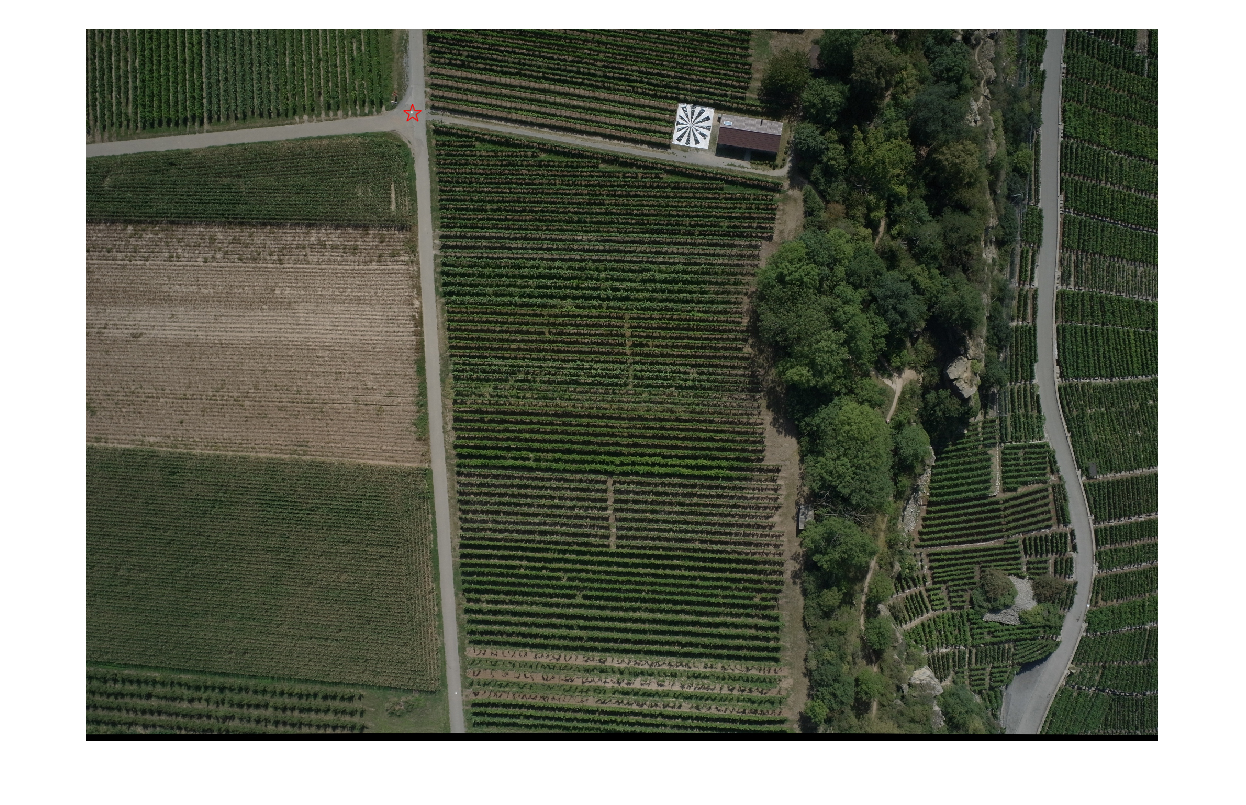
\includegraphics[width=0.45\textwidth]{P2.png}}
\end{figure*}
\newline
\noindent Die Pixel Koordinate von P25 auf linke Bild sind $c = 626.5$, $r = 238.5$, auf Rechte Bild sind $c = 1306.5$, $r = 338.5$ \newline
Über einen räumlichen Vorwärtsschnitt werden die zugehörigen Objektkoordinaten berechnet. zunächst werden die Pixelkoordinaten nach Bildkoordinaten zu rechnen (Innere Orientierung): 
\begin{equation*}
\bm{K} = \begin{bmatrix}
m_x & \ & \ \\
\ & m_y & \ \\
\ & \ & 1 \\  
\end{bmatrix} \begin{bmatrix}
c & \ & p_x \\
\ & c & p_y \\
\ & \ & 1 \\
\end{bmatrix} = \begin{bmatrix}
\alpha_x & \ & x_0 \\
\ & \alpha_y & y_0 \\
\ & \ & 1 \\
\end{bmatrix}
\end{equation*}
Die Kamerakoordinaten werden mit $K$ Matrix und gemessene Pixelkoordinaten gerechnet:
\begin{equation*}
\bm{x_{pix}} = \bm{K} \bm{x_{cam}} \longrightarrow \bm{x_{cam}} = \bm{K^{-1}} \bm{x_{pix}}
\end{equation*}
\newpage
\noindent Hier ist $\bm{K}$ Matrix vorgegeben:
\begin{figure*}[ht]\centering
	\subfigure[$\bm{K}$ Matrix]{
		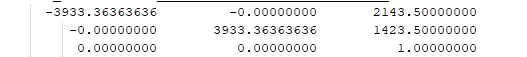
\includegraphics[width=0.9\textwidth]{Inner.png}}
\end{figure*}
\newline
Dann kriegt man die Kamerakoordinaten: 
\begin{equation*}
\begin{bmatrix}
x_1 \\
y_1
\end{bmatrix} = \begin{bmatrix}
0.3857 \\
-0.3013
\end{bmatrix} \qquad \begin{bmatrix}
x_2 \\
y_2
\end{bmatrix} = \begin{bmatrix}
0.2128 \\
-0.2758
\end{bmatrix}
\end{equation*}
Um Vorwärtsschnitt zu machen, rechnet man zuerst die beiden Raumstrahlen $v_1$ und $v_2$:
\begin{equation*}
\bm{v_1} = \bm{R_1^T} \begin{bmatrix}
x_1 \\
y_1 \\
1 
\end{bmatrix} \qquad \bm{v_2} = \bm{R_2^T} \begin{bmatrix}
x_2 \\
y_2 \\
1 
\end{bmatrix}
\end{equation*}
Die beide Rotationsmatrix sind auch gegeben: 
\begin{figure*}[ht]\centering
	\subfigure[$\bm{R_1}$]{
		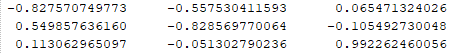
\includegraphics[width=0.45\textwidth]{R1.png}}
	\subfigure[$\bm{R_2}$]{
		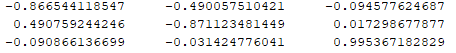
\includegraphics[width=0.45\textwidth]{R2.png}}
\end{figure*}
\newline
$\bm{d}$ ist die Kreuzprodukt zwischen beiden Raumstrahlen: $\bm{d} =\bm{v_1} \times \bm{v_2}$ und $b$ ist Bildbasis: $\bm{b} = \bm{X_{02}} - \bm{X_{01}}$ \newline
Danach kann man folgede Lineargleichung lösen: ($\bm{\lambda^T} = [\lambda_1\ \ \lambda_2 \ \ \lambda_d]$)
\begin{equation*}
\left[\bm{v_1}\ \ \bm{v_2}\ \ \bm{b}\right] \ \bm{\lambda} = \bm{b} \longrightarrow \bm{\lambda} = \left[\bm{v_1}\ \ \bm{v_2}\ \ \bm{b}\right]^{-1} \bm{b}
\end{equation*}
Die Objektkoordinaten kann man dann rechnen:
\begin{gather*}
\bm{P} = \bm{X_{01}} + \lambda_1 \bm{v_1} + \frac{1}{2} \lambda_d \bm{d} \\
\bm{P} = \bm{X_{02}} - \lambda_2 \bm{v_2} - \frac{1}{2} \lambda_d \bm{d} \\
\end{gather*}
\begin{figure*}[ht]\centering
	\subfigure[Zeichnung]{
		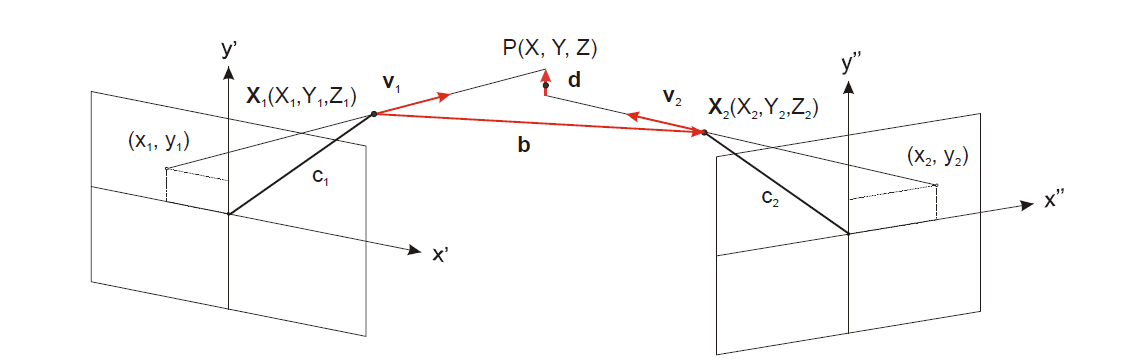
\includegraphics[width=0.5\textwidth]{vorwart.png}}
\end{figure*}
\newpage
\begin{equation*}
\bm{P} = \begin{bmatrix}
X \\
Y \\
Z
\end{bmatrix} = \begin{bmatrix}
513047.865 \\
5427704.457\\
325.592\\
\end{bmatrix}
\end{equation*}
\section{Rücktransformation}
Die vorgegebene Koordinate von P25 ist:
\begin{figure*}[ht]\centering
	\subfigure[Objektkoordinate]{
		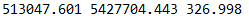
\includegraphics[width=0.4\textwidth]{ObjKoor.png}}
\end{figure*}
\newline
Um die Pixelkoordinaten zu rechnen, baut man an Anfang ein $\bm{P}$ Matrix an:
\begin{equation*}
\bm{P} = \bm{K} \left[ \bm{R} \ \ -\bm{R} \cdot \bm{X}_0\right]
\end{equation*}
Pixelkoordinaten werden durch $\bm{x} = \bm{P} \bm{X}$ gerechnet, wobei $\bm{X}$ homogene Objektkoordinate und $\bm{x}$ homogene Pixelkoordinate sind, dann werden $\bm{x}$ normalisiert: 
\begin{equation*}
\bm{x_1} = \begin{bmatrix}
626.0374 \\
236.2401
\end{bmatrix} \qquad \bm{x_2} = \begin{bmatrix}
1298.9175 \\
332.2546
\end{bmatrix}
\end{equation*}
Diese Ergebnisse passen genau die gemessene Pixelkoordinaten. 
\end{document}